\chapter{Scheduling con Shared Memory}
Finora abbiamo osservato il problema dello \textit{scheduling} con certi vincoli, tra cui: \textbf{\textit{single core}}, \textbf{nessun vincolo} e con nessuna memoria condivisa tra i processi. Andiamo ora ad alleggerire i vincoli e introduciamo il problema della \textbf{concerrenza} per il problema dello \textit{scheduling}.
\begin{figure}[h]
    \centering
    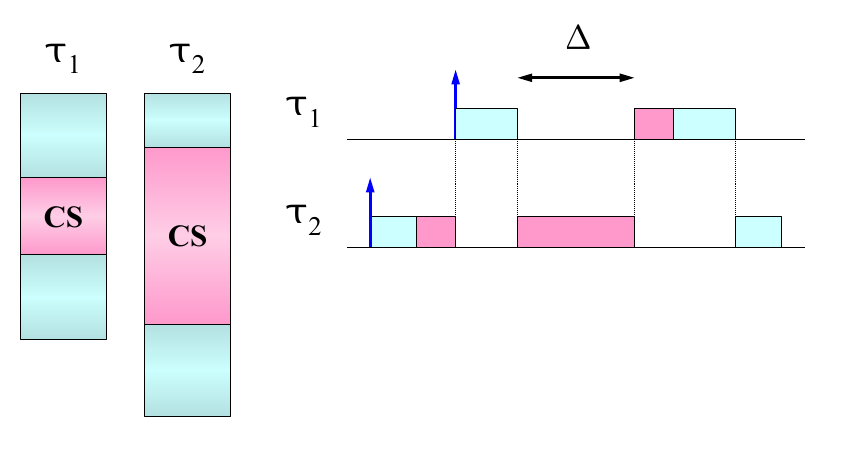
\includegraphics[width=0.5\textwidth]{img/conc_sched_1}
\end{figure}
\\
Consideriamo due task $\tau_1, \tau_2$ che hanno una sezione critica identificata nell'immagine da \textit{CS} e abbiamo che la $P(\tau_1) > P(\tau_2)$. Notiamo che $r_2 < r_1$ e quindi viene attivato prima il task $\tau_2$ in questo modo il task inizia entra nella sezione critica e prende possesso del \textit{mutex} a quel punto il task $\tau_1$ si risveglia e \textit{preempta} $\tau_2$ che però non ha ancora rilasciato il \textit{mutex} quindi quando deve entrare nella sezione critica dovrà mettersi in attesa che il \textit{mutex} venga rilasciato. Dall'immagine sembra che il \textbf{tempo massimo di bloccaggio}, quindi $\Delta$ sarà al massimo uguale alla lunghezza della sezione critica di $\tau_2$, ma nel caso generale possiamo dire che il \textit{blocking delay} è \textbf{\textit{unbounded}}. Andiamo a definire la \textbf{\textit{Priority Inversion}} ovvero che un task ad alta priorità venga bloccato da un task a più bassa priorità per un periodo di tempo \textit{unbounded}. La soluzione a questo problema è quella di introdurre un \textbf{\textit{concurrency control protocol}} per accere alle sezioni critiche.
\begin{figure}[h]
    \centering
    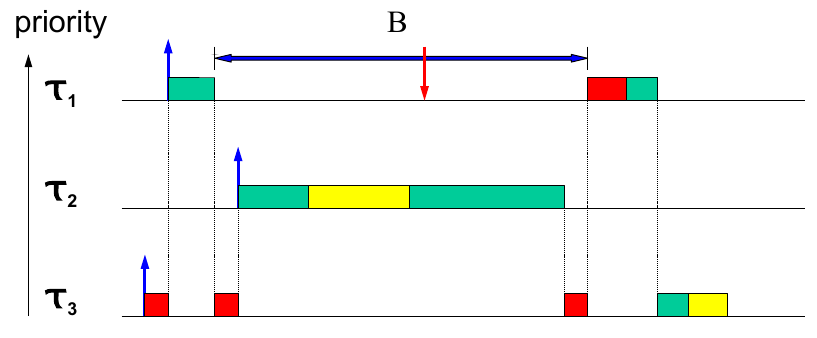
\includegraphics[width=0.5\textwidth]{img/conc_sched_2}
    \caption{\textit{priority inversion}}
\end{figure}
\\
In questa figura possiamo notare che il \textit{task set} è composto da $\mathcal{T} = \{\tau_1, \tau_2, \tau_3\}$ dove $P(\tau_1) > P(\tau_2) > P(\tau_3)$, ma il \textit{request time} sarà $r_3 < r_1 < r_2$. Identifichiamo come le zone rosse e gialle siano le \textit{critical sections}. Osserviamo che il \textit{mutex} della sezione rossa viene ``preso'' da $\tau_3$ che non avendolo ancora rilasciato metterà a dormire il task $\tau_1$, ma siccome durante l'esecuzione della sezione critica rossa il task $\tau_3$ verrà \textit{preemptato} dal task $\tau_2$ che ha priorità maggiore, lasciando però addormentato il task $\tau_1$ che quindi avrà un \textbf{\textit{deadline miss}}. \\
\textbf{\textit{Resource Access Protocols}}
\begin{itemize}
    \item \textbf{\textit{Non Preemptive Protocol} (NPP)}
    \item \textbf{\textit{Highest Locker Priority} (HLP)}
    \item \textbf{\textit{Priority Inheritance Protocol} (PIP)}
    \item \textbf{\textit{Priority Ceiling Procol} (PCP)}
    \item \textbf{\textit{Stack Resource Policy} (SRP)}
\end{itemize}
\newpage
\section{Non Preempive Protocol}
La \textit{preemption} è proibilta nelle sezioni critiche. Ha un'implementazione semplice, nel momento in cui un task entra in una sezione critica la sua priorità viene modificata e portata al massimo possibile. Lo svantaggio più problematico è quello che nel caso incui un task ad alta priorità non abbia sezioni critiche può essere bloccato da questo tipo di controllo.
\begin{figure}[h]
    \centering
    \begin{minipage}[t]{0.45\textwidth}
        \centering
        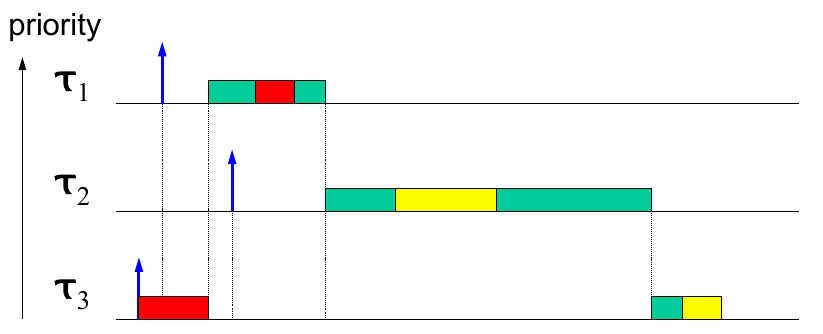
\includegraphics[width=\textwidth]{img/npp}
        \caption{$P_{CS} = max\{P_1, ..., P_n\}$}
    \end{minipage}
    \begin{minipage}[t]{0.45\textwidth}
        \centering
        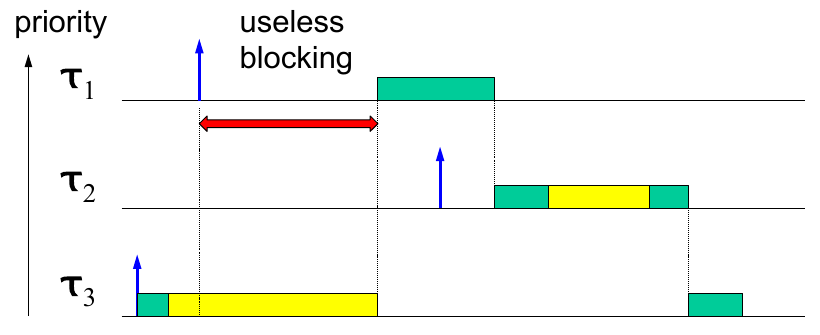
\includegraphics[width=\textwidth]{img/npp_2}
        \caption{NPP troppo forte}
    \end{minipage}
\end{figure}

\section{Highest Locker Priority}
Quando un task entra nella sezione critica ottiene la priorità più alta su le priorità dei task che condividono quella sezione critica. Ha un'implementazione semplice, il task viene bloccato sul tentativo di \textit{preemption} non quando cerca di entrare nella sezione critica. Viene anche chiamato \textbf{\textit{Immediate Priority Ceiling}}.
\begin{figure}[h]
    \centering
    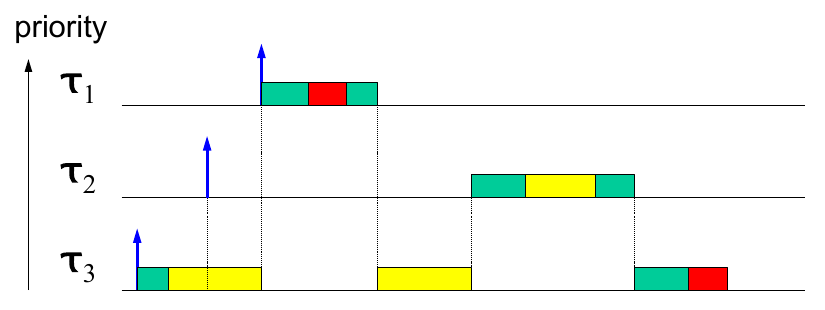
\includegraphics[width=0.5\textwidth]{img/hlp}
\end{figure}
\\
In questo caso la $P_{CS} = max\{P_k \; | \; \tau_k \text{ uses } \mathbf{CS}\}$ in questo caso se $\tau_2$ è bloccato, ma $\tau_1$ può comunque eseguire andando a \textit{preemptare} $\tau_3$. Può esserci una casistica in cui utilizzare il \textit{highest locker priority} è sconveniente, ovvero quando un task $\tau_i$ ha due rami, in uno è presente una sezione critica, mentre nell'altro no, come possiamo differenziarlo a priori per definire quali sono i task con quelle predefinite sezioni critiche.

\section{Priority Inheritance Protocol}
Un task in una \textit{critical section} aumenta la sua priorità solo se blocca altri task, oppure, un task in una sezione critica eredita la priorità maggiore delle priorità dei task bloccati sulla sezione critica. \[P_{CS} = max\{P_k \; | \; \tau_k \text{ blocked on CS}\}\]
\begin{figure}[h]
    \centering
    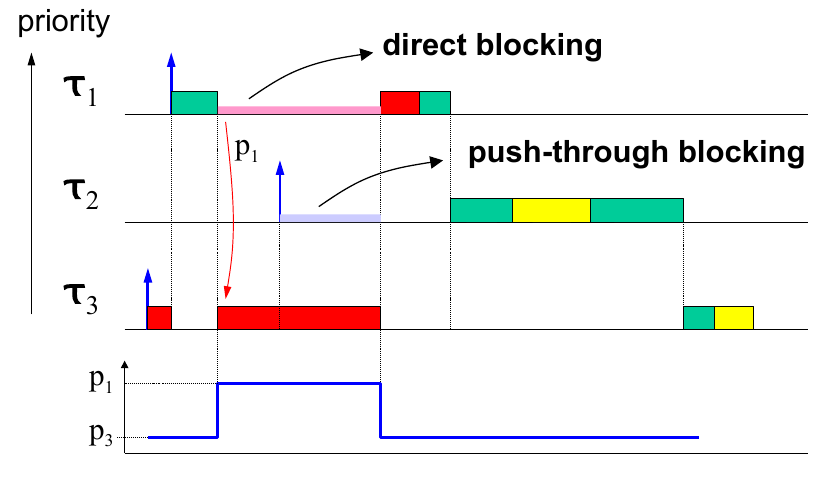
\includegraphics[width=0.7\textwidth]{img/pip}
\end{figure}
\\
In questa rappresentazione possiamo identificare due tipologie ritardi:
\begin{itemize}
    \item \textbf{\textit{direct blocking}}: un task che è bloccato su un semaforo bloccato.
    \item \textbf{\textit{push-through blocking}}: un task è bloccato perché un task a più bassa priorità ha ereditato un priorità maggiore.
\end{itemize}
Definiamo come \textbf{\textit{blocking}} su un task $\tau_i$ il ritardo causato da un task a più bassa priorità. Un task $\tau_i$ può essere bloccato da quei semafori utilizzati da task con priorità inferiore che possono essere direttamente confivise con $\tau_i$ (\textbf{\textit{direct blocking}}) oppure confivisi con task che hanno priorità maggiore rispetto a $\tau_i$ (\textbf{\textit{push-through blocking}}). \\
\textbf{Teorema [bloccaggio sulle risorse]}: un task $\tau_i$ può essere bloccato al massimo una volta per ognuno di quei semafori. \\
Se definiamo $n$ come il numero di task a più bassa priorità che può bloccare $\tau_i$ e $m$ il numero dei semafori su cui $\tau_i$ può essere bloccato. \\
\textbf{Teorema [bloccaggio sul tempo]}: $\tau_i$ può essere bloccato al massimo per la durata di $min(n, m)$ sulle sezioni critiche.
\begin{center}
    \begin{tabular}{ c | c }
        \textcolor{green}{\textbf{Vantaggi}} & \textcolor{red}{\textbf{Svantaggi}} \\
        \textbf{-} è trasparente al programmatore & \textbf{-} non rimuove \textit{deadlock} e \textit{chained blocking} \\
        \textbf{-} evita le \textit{priority inversion} &  \\
    \end{tabular}
\end{center}
\begin{figure}[h]
    \centering
    \begin{minipage}[t]{0.45\textwidth}
        \centering
        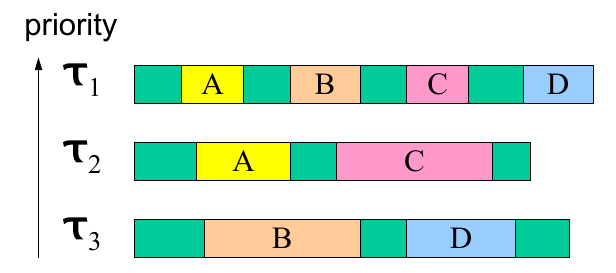
\includegraphics[width=\textwidth]{img/pip_2}
    \end{minipage}
    \begin{minipage}[t]{0.45\textwidth}
        \centering
        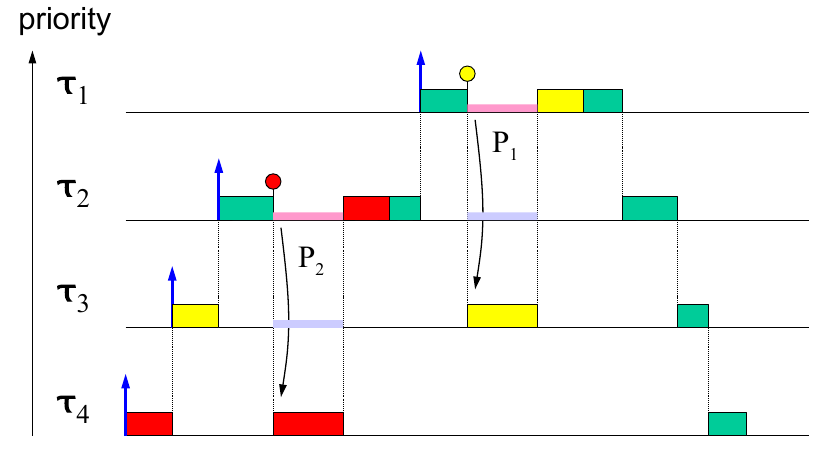
\includegraphics[width=\textwidth]{img/pip_3}
    \end{minipage}
\end{figure}
Il task $\tau_1$ può essere bloccato una volta da $\tau_2$ (o nella sezione critica $A_2$ o $C_2$) e una volta da $\tau_3$ (o nella sezione critica $B_3$ oppure $D_3$), $\tau_2$ può essere bloccato una volta in $\tau_3$ (o nella sezione critica $B_3$ o $D_3$), mentre $\tau_3$ non può essere bloccato. \\
Nel \textbf{\textit{chained blocking}} con \textbf{PIP} $\tau_i$ può essere bloccato al massimo una volta da ogni task con più bassa priorità.
\newpage
\section{Priority Ceiling Protocol}
Il \textit{priority ceiling protocol} può essere visto come il \textbf{PIP} ma ha un \textit{access test}, un task può entrare in una sezione critica solo se è libera e non c'è il rischio di un \textit{chainged blocking}, per implementarlo il task viene bloccato sull'ingresso della \textit{critical sections} [\textit{ceiling blocking}]. \\
Definiamo il \textbf{\textit{ceiling}} di una risorsa come la priorità più alta di tutti quei task che richiederanno accesso ad una certa risorsa. Viene assegnato ad ogni semaforo $s_k$ un \textit{ceiling}: $C(s_k) = max{P_j \; | \; T_j \; \text{uses} \; s_k}$. Un task $\tau_i$ può accedere ad una \textit{critical sections} se e solo se \[P_i > max\{C(s_k) \; | \; s_k \text{ locked by task } \neq \tau_i\}\]
\begin{figure}[h]
    \centering
    \begin{minipage}[t]{0.45\textwidth}
        \centering
        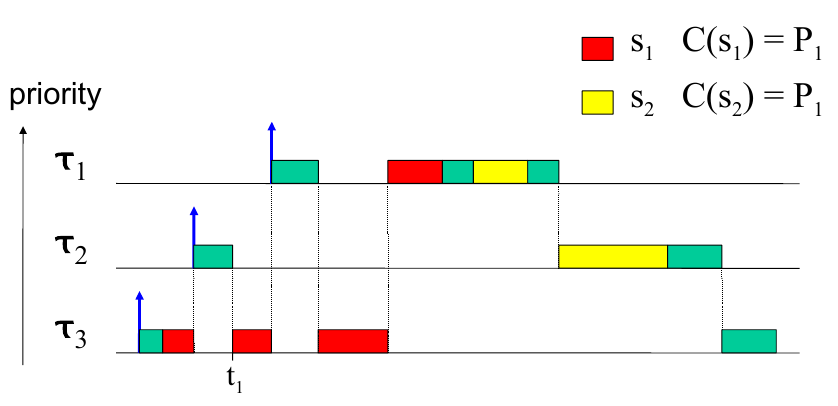
\includegraphics[width=\textwidth]{img/pcp_1}
    \end{minipage}
    \begin{minipage}[t]{0.45\textwidth}
        \centering
        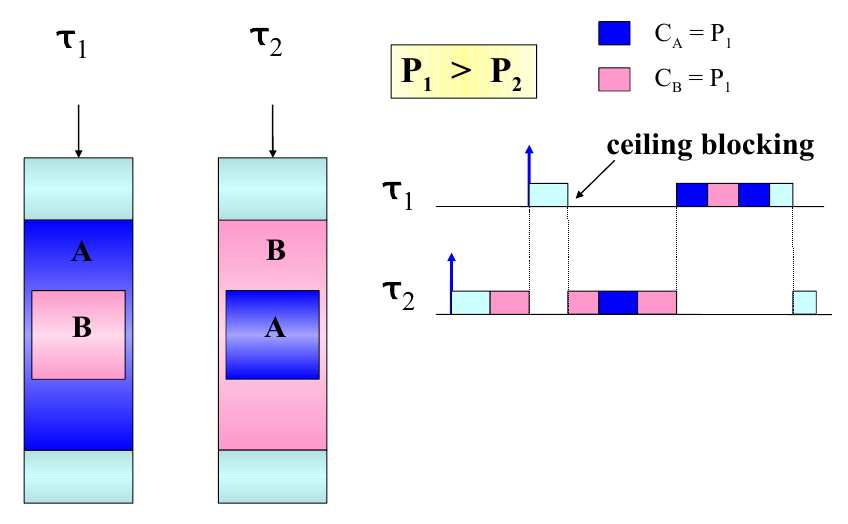
\includegraphics[width=\textwidth]{img/pcp_2}
    \end{minipage}
\end{figure}
\\
Nella prima figura è possibile osservare come il $t_1$ il task $\tau_2$ viene bloccato da \textit{PCP} in quando la priorità di $\tau_2$ è minore del valore del \textit{ceiling} sulla risorsa rossa ($C(s_1) = P_1$).
\begin{center}
    \begin{tabular}{ p{7.25cm} | p{7.25cm} }
        \textcolor{green}{\textbf{Vantaggi}} & \textcolor{red}{\textbf{Svantaggi}} \\
        \textbf{-} il bloccaggio su una sezione critica è ridotto ad una sola & \textbf{-} non è trasparente al programmatore bisogna definire per ogni semaforo il suo \textit{ceiling} \\
        \textbf{-} evita i \textit{deadlock} [vedi figura a destra] &  \\
    \end{tabular}
\end{center}
Ricordiamo che \textit{PCP} è un \textbf{\textit{resource access protocol}} dobbiamo ora scegliere il \textit{scheduling algorithm}, l'idea è quella di calcolare il \textbf{\textit{maximum blocking times}} $B_i$ per ogni task. Per \textit{rate monotonic - RM} \[\forall \tau \in \mathcal{T} \sum_{k=1}^{i-1}\frac{C_k}{T_k} + \frac{C_i + B_i}{T_i} \leq i \cdot (\sqrt[i]{2} - 1)\]
Mentre per \textit{earliest deadline first - EDF} \[\forall \tau \in \mathcal{T} \sum_{k=1}^{i-1}\frac{C_k}{T_k} + \frac{C_i + B_i}{T_i} \leq 1\]
\textcolor{yellow}{\textbf{Esercizio}}

\newpage
\section{Stack Resource Policy (SRP)}
Possiamo vederlo come \textit{HLP} applicato ad \textit{EDF}, ad ogni \textit{hard task} (periodici e sporadici) gli viene assegnato:
\begin{itemize}
    \item una \textit{priority} $p_i$.
    \item un \textit{preemption level} $\pi_i$, possiamo considerarla una priorità fittizia visto che in \textit{EDF} non esistono \[\pi_i = \frac{1}{T_i}\]
    \item ad ogni risorsa $r_i$ viene assegnato un \textit{ceiling} statico definito come: $C(r_k) = max_i\{\pi_i \; | \; \tau_i \text{ needs } r_k\}$
    \item e viene definito un \textbf{\textit{dynamic system ceiling}} come: $\Pi_s(t) = max\{C(r_k) \; | \; R_k \text{ è occupata in t}\}$
\end{itemize}
Il \textbf{\textit{SRP}} ha come ``regola'' per l'ammissione all'esecuzione i task che enuncia: un \textit{job} con priorità più alta è autorizzato ad eseguire se il \textit{preemption level} è maggiore del \textit{system ceiling}. Questo permette che una volta che un thread è in esecuzione non verrà mai bloccato fino al completamento e potrà essere \textit{preemptato} solamente da thread con priorità maggiore. \textit{SRP} previene i deadlock e prviene le \textit{preemption} ``inutili'', infatti nessun task può essere \textit{preemptato} se non ci sono risorse sufficienti. Permette di avere un tempo massimo di bloccaggio $B_i$ \textbf{limitato} definendolo come la massima lunghezza della sezione critica del task con priorità minore che ha accesso ad una risorsa condivisa con un task che ha priorità uguale o maggiore. Un \textit{task set} $\mathcal{T}$ può essere \textit{schedulato} sotto \textit{EDF + SRP} se: \[\forall i \; 1 \leq i \leq n \qquad (\sum_{k=1}^i \frac{C_k}{T_k}) + \frac{B_i}{T_i} \leq 1\]
\textbf{\textit{SRP}} permette hai task di \textbf{condividere} un singolo \textbf{\textit{user-level stack}}.